\section{Single Pulse Delay MLE}
\label{sec:Single-Pulse-Delay-Estimation}

A single continuous pulse \(t\mapsto s(t)\) is sent from the transmitter and, assuming that the pulse retains the same shape and extension, we define the detected pulse at element \(r\) as:
\begin{equation}
\begin{aligned}
f_r(t)
&=\lambda_{b,r}+\lambda_{s,r} \, s(t-\delta_{r})\\
&=\lambda_{b,r}+\lambda_{s,r} \, s(t-\tau_{F}-\tau_{0r})\\
&=\lambda_{b,r}+\lambda_{s,r} \, s(t-\delta_{0}-\tau_{0r}),
\end{aligned}
\label{eq:thetriade}
\end{equation}
where \(\delta_r\) is the \textbf{total time delay} from the source to element \(r\), \(\tau_F\) is the common \textbf{time of flight} (TOF) and we chose element \(r=0\) to be the reference within the array. The \textbf{relative time delay} is defined as \(\tau_{0r}=\delta_r-\delta_0\) \(\forall r\in\{0,\ldots,R-1\}\), \(\lambda_{s,r}\) is the amplitude, and \(\lambda_{b,r}\) is the background noise floor.

\noindent
We are going to assume that the extension of the pulse \(t\mapsto s(t)\) is an \textbf{integer multiple of a time slot} \(nT_s\), with \(n \in \mathbb{Z}_{\geq1}\), meaning that \(\forall t\notin [0,nT_s], s(t)=0\).
\noindent
If we assume \(t \mapsto f_r(t)\) to model the intensity of the incident light detected at \textbf{element} \(r\), we can then model the number of photons arriving at every time \textbf{slot} \(i\) as a non-homogeneous Poisson random process with
\begin{equation}
\begin{aligned}
x_r[i]
& \sim \operatorname{Poi}\left(\psi_{i,r}(\delta_r)\right),
\end{aligned}
\end{equation}
where
\begin{equation}
\psi_{i,r}(\delta_r) = \int_{iT_s}^{(i+1)T_s}f_r(t) \di t.
\end{equation}

\noindent
Using the definitions in~\eqref{eq:thetriade} we can see that:
\begin{equation}
\psi_{i,r}(\delta_r)
= \int_{iT_s}^{(i+1)T_s} \left[ \lambda_{b,r}+\lambda_{s,r} \, s(t-\delta_{r}) \right] \di t
= \lambda_{b,r} T_s+\lambda_{s,r}\, S_i\left(\delta_r\right),
\label{eq:model}
\end{equation}
where we used the definition
\begin{equation}
S_i(\delta_r) = \int_{iT_s}^{(i+1)T_s} s(t-\delta_r) \di t.
\label{eq:thebigs}
\end{equation}

\noindent
Something maybe worth noting is that, for a general pulse \(t\mapsto s(t)\), the rate of change of the delay-dependent intensity function of the Poisson process is:
\begin{equation}
\begin{aligned}
\frac{\partial \psi_{i,r}(\delta_r)}{\partial \delta_r}
= \lambda_{s,r}\,\frac{\partial S_i(\delta_r)}{\partial \delta_r}
= \lambda_{s,r}
\left[-s\left((i+1)T_s-\delta_r\right)+s\left(iT_s-\delta_r\right)\right].
\end{aligned}
\label{eq:thederivative}
\end{equation}

\noindent
If we assume the \textbf{observation window} \(W\in\mathbb{R}_{\geq0}\) to be an integer multiple of \(T_s\), i.e. \(W=LT_s\) with \(L\in \mathbb{Z}_{\geq1}\), then we must ensure that the delayed pulse is actually fully contained within our observation:
\begin{equation}
W=LT_s>nT_s+\delta_r \quad \forall  r\in\{0,\ldots,R-1\}.
\label{eq:thecondition}
\end{equation}
To recap, with \(r\in\{0,\ldots,R-1\}\) being the \textbf{antenna number}, \(i\in\{0,\ldots,L-1\}\) being the \textbf{slot number} and \(n \in \mathbb{Z}_{\geq1}\) being the integer length of the pulse, the goal is to first estimate the \textbf{total time delays} \((\delta_0,\delta_1,\ldots,\delta_{R-1})\) and then the TDOAs \((\tau_{00},\tau_{01},\ldots\tau_{0(R-1)})=(\delta_0-\delta_0,\delta_1-\delta_0,\ldots,\delta_{R-1}-\delta_0)\) from the photon-starved Poisson model:
\begin{equation}
x_r[i]\sim \operatorname{Poi}\left(\psi_{i,r}(\delta_r)\right)
\quad
\text{with}
\quad
\psi_{i,r}(\delta_r)=\lambda_{b,r} T_s+\lambda_{s,r}\, S_i\left(\delta_r\right).
\end{equation}

\noindent
If we define \(t\mapsto s(t)\) as a rectangular function with \(n \in \mathbb{Z}_{\geq1}\):
\begin{equation}
s(t)=\operatorname{rect}_{(nT_s)}(t)=
\begin{cases}
1 & 0\leq t \leq nT_s\\ 
0 & \text {else},
\end{cases}
\label{eq:rectmodel}
\end{equation}
then from~\eqref{eq:thetriade} we have:
\begin{equation}
f_r(t)=\lambda_{b,r}+\lambda_{s,r} \operatorname{rect}_{(nT_s)}(t-\delta_{r}) =
\begin{cases}
\lambda_{s,r}+\lambda_{b,r} & \delta_{r}\leq t \leq \delta_{r}+nT_s\\ 
\lambda_{b,r} & \text {else},
\end{cases}
\label{eq:respect}
\end{equation}
represented in~\Cref{fig:single}. We can then see from~\eqref{eq:thebigs} that
\begin{equation}
\begin{aligned}
S_i\left(\delta_r\right)
= &\int_{iT_s}^{(i+1)T_s} \operatorname{rect}_{(nT_s)}(t-\delta_{r}) \di t\\
= & \max \left[0, \min \left((i+1) T_s, \delta_r+n T_s\right)-\max \left(i T_s, \delta_r\right)\right], 
\end{aligned}
\label{eq:staroba}
\end{equation}
and hence from~\eqref{eq:model}:
\begin{equation}
\begin{aligned}
\psi_{i,r}(\delta_r)
= \lambda_{b,r}T_s+
\lambda_{s,r}\max \left[0, \min \left((i+1) T_s, \delta_r+n T_s\right)-\max \left(i T_s, \delta_r\right)\right].
\end{aligned}
\label{eq:bah}
\end{equation}

\begin{figure}[!t]
\centering
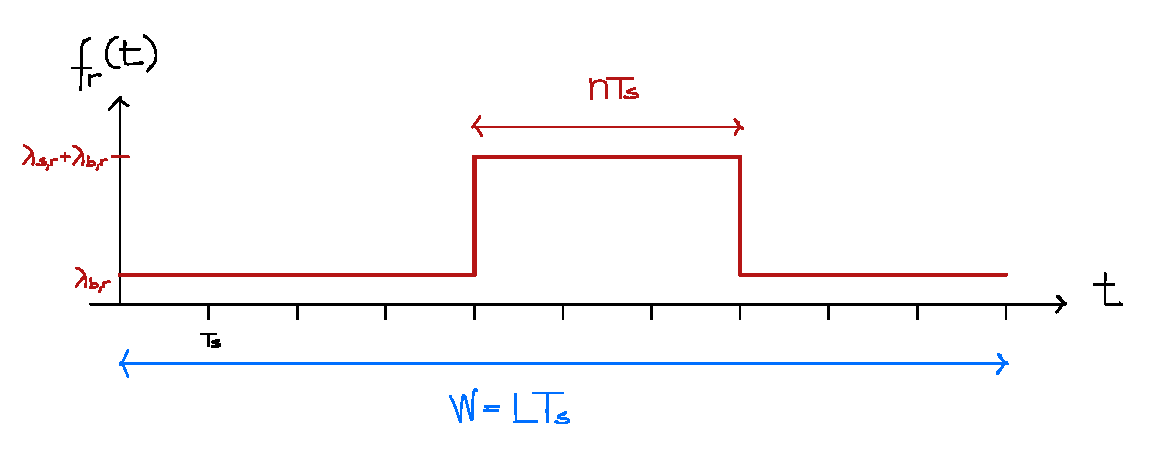
\includegraphics[
  width=0.9\textwidth,
  keepaspectratio,
  clip,
]{figs/singlepulse.pdf}
\caption[]{Plot of the detected pulse~\eqref{eq:respect}.}
\label{fig:single}
\end{figure}

\noindent
Another possible pulse definition \(t\mapsto s(t)\) could be a Gaussian function with variance \(\sigma^2\), mean \(\mu_s = (nT_s)/2\), and a multiplying constant chosen such that the total energy of the pulse is \(nT_s\):
\begin{equation}
s(t)= \sqrt{\frac{nT_s}{\sigma\sqrt{\pi}}}
\exp\left(-\frac{(t-(nT_s)/2)^2}{2\sigma^2}\right),
\label{eq:gaussianpulse}
\end{equation}
with
\begin{equation}
\begin{aligned}
S_i\left(\delta_r\right)
= &\int_{iT_s}^{(i+1)T_s} \sqrt{\frac{nT_s}{\sigma\sqrt{\pi}}}
\exp\left(-\frac{((t-\delta_r)-(nT_s)/2)^2}{2\sigma^2}\right) \di t\\
= & \sqrt{{n T_s \sigma(\sqrt{\pi}}/{2}) }
\left[
\operatorname{erf}\!\left(\frac{(i+1)T_s-\delta_r-\tfrac{nT_s}{2}}{\sqrt{2}\,\sigma}\right)
-
\operatorname{erf}\!\left(\frac{iT_s-\delta_r-\tfrac{nT_s}{2}}{\sqrt{2}\,\sigma}\right)
\right],
\end{aligned}
\end{equation}
where \(\text{erf}\) is the error function as defined in~\cite{wiki:Error_function}.

\subsection{ML Estimation}\label{sub:MLestimation1}

\noindent
To simplify the notation, in this sub-chapter we are going to look at a \textbf{single receiving antenna first}, denoting the \textbf{total time delay} \(\delta_r\) with \(\delta\) and the number of photons arriving at time slot \(i\), \(x_r[i]\) simply with \(x_i\). In ML estimation no prior distribution \(p_{\delta}\left(\delta\right)\) is assumed to exist and, recalling that we assumed to have a total of \(L\) observations from the observation window \(W\), the estimation rule is:
\begin{equation}
\delta_{\mathrm{ML}} =\underset{\delta}{\argmax} \ell(\delta ; \mathbf{x})
\end{equation}
where \(\ell(\delta ; \mathbf{x})=\log p_{\textbf{x} \mid \delta}\left( x_0, \ldots,x_{L-1} \mid\delta\right)\) is the log-likelihood function with respect to the parameter \(\delta\) of the observation vector \(\mathbf{x}=(x_0,\ldots,x_{L-1})\). The log-likelihood of these \(L\) observations is:
\begin{equation}
\begin{aligned}
\ell(\delta ; \mathbf{x})
= & \log p_{\textbf{x} \mid \delta}\left(x_0, \ldots,x_{L-1} \mid \delta\right)\\
\overset{\text{(a)}}{=} & \log \prod_{i=0}^{L-1} p_{x_i \mid \delta}\left(x_i \mid \delta\right)\\
= & \sum_{i=0}^{L-1} \log p_{x_i \mid \delta}\left(x_i \mid \delta\right) \\
= & \sum_{i=0}^{L-1} \log \left(\frac{\exp(-\psi_i(\delta))(\psi_i(\delta))^{x_i}}{x_{i}!} \right)\\
= & \sum_{i=0}^{L-1} x_i \log \left( \psi_i(\delta)\right) -\psi_i(\delta)-\log \left(x_{i}!\right),
\end{aligned}
\label{eq:the_true_one}
\end{equation}
where in step (a) we used the conditional independence between the elements of the vector \(\mathbf{x}\). Note that given the model~\eqref{eq:model}, with~\eqref{eq:rectmodel} and the \textbf{condition}~\eqref{eq:thecondition}:
\begin{equation}
\begin{aligned}
\sum_{i=0}^{L-1}\psi_i(\delta)
& = \sum_{i=0}^{L-1}
\int_{iT_s}^{(i+1)T_s} \left[ \lambda_{b}+\lambda_{s} \, s(t-\delta) \right] \di t\\
& = \int_{0}^{LT_s} \left[ \lambda_{b}+\lambda_{s} \, s(t-\delta) \right] \di t\\
& = \int_{0}^{LT_s} \left[ \lambda_{b}+\lambda_{s} \, \operatorname{rect}_{(nT_s)}(t-\delta) \right] \di t\\
& =LT_s\lambda_b+nT_s\lambda_s.
\end{aligned}
\end{equation}

\noindent
Therefore, we have:
\begin{equation}
\begin{aligned}
\delta_{\mathrm{ML}} 
= & \underset{\delta}{\argmax}
\left[
\sum_{i=0}^{L-1} x_i \log \left( \psi_i(\delta)\right)
-\sum_{i=0}^{L-1}  \psi_i(\delta)
-\sum_{i=0}^{L-1}  \log \left(x_{i}!\right)
\right]
=\underset{\delta}{\argmax} 
\sum_{i=0}^{L-1} x_i \log \left( \psi_i(\delta)\right).
\end{aligned}
\label{eq:sweetsix}
\end{equation}

\noindent
The objective is to maximize the log-likelihood with respect to \(\delta\), and if the log-likelihood is both differentiable and concave, the problem boils down to simply finding the zero of the derivative of the log-likelihood with respect to \(\delta\). In our case, the function is only differentiable and concave in the open interval \((iT_s,(i+1)T_s)\) corresponding to the time slot \(i,\;\forall i\in\{0,\ldots,L-1\}\).

\noindent
We then take the derivative with of the log-likelihood over the interval \(\delta \in(iT_s,(i+1)T_s)\) using~\eqref{eq:thederivative},~\eqref{eq:rectmodel} and~\eqref{eq:bah}:
\begin{equation}
\begin{aligned}
\frac{\partial}{\partial \delta} \ell(\delta ; \mathbf{x})
= &\frac{\partial}{\partial \delta}\sum_{i=0}^{L-1} x_i \log \left( \psi_i(\delta)\right)
= \sum_{i=0}^{L-1}x_i\frac{ \frac{\partial}{\partial \delta}\psi_i(\delta)}{\psi_i(\delta)}
= \sum_{i=0}^{L-1}x_i\frac{\lambda_{s}\,\frac{\partial S_i(\delta)}{\partial \delta}}{\psi_i(\delta)}\\
= &\sum_{i=0}^{L-1}x_i\frac{\lambda_{s}
\left[-s\left((i+1)T_s-\delta\right)+s\left(iT_s-\delta_r\right)\right]}{\psi_i(\delta)}\\
= &\sum_{i=0}^{L-1}x_i\frac{\lambda_{s}
\left[-\operatorname{rect}_{(nT_s)}\left((i+1)T_s-\delta\right)+\operatorname{rect}_{(nT_s)}\left(iT_s-\delta\right)\right]}{\psi_i(\delta)}\\
= &\sum_{i=0}^{L-1}x_i\frac{\lambda_{s}
\left[-\operatorname{rect}_{(nT_s)}\left((i+1)T_s-\delta\right)+\operatorname{rect}_{(nT_s)}\left(iT_s-\delta\right)\right]}
{\lambda_{b}T_s+\lambda_{s}\max \left[0, \min \left((i+1) T_s, \delta+n T_s\right)-\max \left(i T_s, \delta\right)\right]}.
\end{aligned}
\label{eq:ilterrore}
\end{equation}

\noindent
If one looks at this sum of functions,~\eqref{eq:ilterrore} can be divided into two kinds of intervals: the first \(L-n\) intervals, from \((0,T_s)\) up to \( \left((L-n-1)T_s,(L-n)T_s\right)\) and the last \(n\) from \(((L-n)T_s,(L-n+1)T_s)\) up to \( \left((L-1)T_s,LT_s\right)\). The result of~\eqref{eq:ilterrore} is then:
\begin{equation}
\begin{aligned}
\frac{\partial}{\partial \delta} \ell(\delta ; \mathbf{x}) =
\begin{cases}
x_{i+n} \frac{\lambda_s}{\left(\lambda_s \delta-i \lambda_s T_s\right)+\lambda_b T_s}
-x_i \frac{\lambda_s}{\left(-\lambda_s \delta+(i+1) \lambda_s T_s\right)+\lambda_b T_s} 
& i\in\{0, \ldots, L-n-1\} \\ 
-x_i \frac{\lambda_s}{\left(-\lambda_s \delta+(i+1) \lambda_s T_s\right)+\lambda_b T_s} 
& i\in\{L-n, \ldots, L-1\}.
\end{cases}
\end{aligned}
\label{eq:plutone}
\end{equation} 

\medskip
\noindent\rule{\linewidth}{0.4pt} % width, thickness
\medskip
If the rectangular function is not a multiple of the time slots i.e. \(n \notin \mathbb{Z}_{\geq1}\), result~\eqref{eq:plutone} becomes:
\begin{equation}
\begin{aligned}
\frac{\partial}{\partial \delta} \ell(\delta ; \mathbf{x}) 
&=
\begin{cases}
x_{i+\lfloor n\rfloor} \frac{\lambda_s}{\left(\lambda_s \delta-(i-n\,\text{mod}\,1) \lambda_s T_s\right)+\lambda_b T_s}\\
+x_{i+\lceil n\rceil} \frac{\lambda_s}{\left(\lambda_s \delta-(i+n\,\text{mod}\,1) \lambda_s T_s\right)+\lambda_b T_s}\\
-x_i \frac{\lambda_ s}{\left(-\lambda_s \delta+(i+1) \lambda_s T_s\right)+\lambda_b T_s} 
& i\in\{0, \ldots, L-\lceil n\rceil-1\}\
\end{cases}\\
&=
\begin{cases}
-x_i \frac{\lambda_s}{\left(-\lambda_s \delta+(i+1) \lambda_s T_s\right)+\lambda_b T_s} 
& \qquad \quad \; i\in\{L-\lceil n \rceil, \ldots, L-1\}.
\end{cases}
\end{aligned}
\end{equation} 
\medskip
\noindent\rule{\linewidth}{0.4pt} % width, thickness
\medskip

\noindent
We now note that actually by condition~\eqref{eq:thecondition} we have \(\delta<(L-n)T_s\), meaning that delay is by construction must be in the first \(L-n\) intervals. Therefore, concentrating on \(i\in\{0, \ldots, L-n-1\}\), we find the possible candidate solutions in each time slot interval, by finding the zero of~\eqref{eq:plutone}:
\begin{gather}
\frac{\lambda_s x_{i+n}}{\left(\lambda_s \delta_{\mathrm{ML}, i}-i \lambda_s T_s\right)+\lambda_b T_s}
=\frac{\lambda_s x_i}{\left(-\lambda_s \delta_{\mathrm{ML}, i}+(i+1) \lambda_s T_s\right)+\lambda_b T_s},\\
\left(-\delta_{\mathrm{ML}, i}+(i+1) T_s+\frac{\lambda_b}{\lambda_s} T_s\right) x_{i+n}
=x_i\left(\delta_{\mathrm{ML}, i}-i T_s+\frac{\lambda_b}{\lambda_s} T_s\right),\\
- x_{i+n}\delta_{\mathrm{ML}, i}+x_{i+n}\left((i+1) T_s+\frac{\lambda_b}{\lambda_s} T_s\right)
=x_i \delta_{\mathrm{ML}, i}+x_i\left(\frac{\lambda_b}{\lambda_s} T_s-i T_s\right),
\end{gather}
and so:
\begin{equation}
\begin{aligned}
\delta_{\mathrm{ML}, i}
&=T_s\left[\frac{x_{i+n}\left(i+1 +\frac{\lambda_b}{\lambda_s} \right)+x_i\left(i -\frac{\lambda_b}{\lambda_s} \right)}{x_i+x_{i+n}}\right].
\end{aligned} 
\label{eq:estimator}
\end{equation}
Estimates are valid only if \(iT_s<\delta_{\mathrm{ML}, i}<(i+1)T_s\) otherwise they are set equal to \(iT_s\) or \((i+1)T_s\). The final estimate is then found as the maximum between the interval estimates:
\begin{equation}
\delta_{\mathrm{ML}}=\underset{i}{\argmax} \; \ell\left(\delta_{\mathrm{ML}, i} ; \mathbf{x}\right) \quad i\in\{0, \ldots, L-n-1\}.
\label{eq:afterestimator}
\end{equation}

\subsection{Cramér-Rao Bound}
The bias-variance decomposition of the mean squared error is:
\begin{equation}
\operatorname{MSE}(\hat{\delta};\delta)=\operatorname{Var}(\hat{\delta};\delta)+\operatorname{Bias}(\hat{\delta};\delta)^2 ,
\end{equation}
for unbiased estimators we have :
\begin{equation}
\operatorname{Var}(\hat{\delta};\delta) \geq \frac{1}{\mathcal{I}(\delta)},
\end{equation}
while for biased estimators:
\begin{equation}
\operatorname{Var}(\hat{\delta};\delta) \geq \frac{(1+\frac{\partial}{\partial \delta}\operatorname{Bias}(\hat{\delta};\delta))^2}{\mathcal{I}(\delta)},
\end{equation}
where \(\mathcal{I}(\delta)\) is the Fisher information of the random variable \(\mathbf{x}\) with respect to the parameter \(\delta\).

\begin{enumerate}
    \item The maximum likelihood estimate is at least asymptotically unbiased (meaning that as the number of observations increases the bias of the MLE tends to zero). It may be unbiased for any number of observations but it is not a guarantee.
    \item The maximum likelihood estimate is at least asymptotically efficient. As the number of observations increases, the MSE of the MLE tends to the Cramér-Rao bound.
\end{enumerate}

\noindent
\subsubsection{Bias}

\noindent
We first compute the bias of~\eqref{eq:estimator}, always with \(\delta \in(iT_s,(i+1)T_s)\) and with \(i\in\{0, \ldots, L-n-1\}\):
\begin{equation}
\mean{\delta_{\mathrm{ML}, i}}
=
T_s \;
\mean{
\frac{x_{i+n}\left(i+1 +\frac{\lambda_b}{\lambda_s} \right)+x_i\left(i -\frac{\lambda_b}{\lambda_s} \right)}{x_i+x_{i+n}}
}
=
T_s \;
\mean{
\frac{x_{i+n}A_i+x_iB_i}{x_i+x_{i+n}}
},
\label{eq:previously}
\end{equation}
with
\begin{equation}
A_i =i+1 +\frac{\lambda_b}{\lambda_s}
\quad \text{and} \quad
B_i =i -\frac{\lambda_b}{\lambda_s}.
\label{eq:definitions}
\end{equation}

\noindent
Knowing that the disjoint bins of the Poisson process, i.e. the time slots counts \(x_i\) and \(x_{i+n}\), are independent, recalling that 
\begin{equation}
x_i \sim \operatorname{Poi}\left(\psi_i(\delta)\right)
\quad \text{and} \quad
x_{i+n} \sim \operatorname{Poi}\left(\psi_{i+n}(\delta)\right),
\end{equation}
using the notation \(Z=x_i+x_{i+n}\), and the properties of the sum of independent Poisson random variables, we have:
\begin{equation}
x_i \mid Z =q\sim \operatorname{Bin}\left(q,\frac{\psi_{i}(\delta)}{\psi_{i}(\delta)+\psi_{i+n}(\delta)}\right),
\label{eq:thebinomial}
\end{equation}
where \(Y\sim \operatorname{Bin}(q,p)\) is a Binomial random variable with mean \(qp\). 

\noindent
Then we notice that, if \(Z =q\), then \(x_{i+n}=q-x_i\) and we have first:
\begin{equation}
\frac{x_{i+n}A_i+x_iB_i}{x_i+x_{i+n}}=
\frac{A_i x_{i+n}+B_i x_i}{Z}=\frac{A_i(q-x_i)+B_i x_i}{q}=A_i+\left(B_i-A_i\right) \frac{x_i}{q},
\end{equation}
and then for \(q> 0\):
\begin{equation}
\begin{aligned}
\mean{\frac{x_{i+n}A_i+x_iB_i}{Z} \bigg| Z=q}
&=
A_i+\left(B_i-A_i\right) \frac{\mean{x_i\mid Z=q}}{q}\\
&=
A_i+\left(B_i-A_i\right) \frac{q\frac{\psi_{i}(\delta)}{\psi_{i}(\delta)+\psi_{i+n}(\delta)}}{q}\\
&=
A_i+\left(B_i-A_i\right) \frac{\psi_{i}(\delta)}{\psi_{i}(\delta)+\psi_{i+n}(\delta)}\\
&=
\frac{\psi_{i+n}(\delta)A_i+\psi_{i}(\delta)B_i}{\psi_{i+n}(\delta)+\psi_{i}(\delta)}.
\end{aligned}
\label{eq:volevoquesta}
\end{equation}

\noindent
We then notice that for \(\delta \in(iT_s,(i+1)T_s)\):
\begin{equation}
\psi_{i+n}(\delta)=\lambda_s\left( \delta-i T_s\right)+\lambda_b T_s
\quad \text{and} \quad
\psi_{i}(\delta)=\lambda_s\left((i+1) T_s -\delta\right)+\lambda_b T_s,
\end{equation}
and
\begin{equation}
\psi_{i+n}(\delta)+\psi_{i}(\delta)
=\lambda_sT_s+2\lambda_b T_s.
\end{equation}

\noindent
Hence, given~\eqref{eq:volevoquesta} and the definitions~\eqref{eq:definitions} after some algebraic manipulations we get:
\begin{equation}
\mean{\frac{x_{i+n}A_i+x_iB_i}{x_i+x_{i+n}} \bigg| Z=q}
=
\frac{\psi_{i+n}(\delta)A_i+\psi_{i}(\delta)B_i}{\psi_{i+n}(\delta)+\psi_{i}(\delta)}
= \delta\frac{\lambda_s+2\lambda_b}{T_s(\lambda_s+2\lambda_b)}
= \frac{\delta}{T_s}.
\label{eq:theresulting}
\end{equation}

\noindent
Then, assuming that we at least one photon arrives in the sum of the time slots under consideration i.e. \(Z>0\), by the law of total expectation:
\begin{equation}
\begin{aligned}
\mean{\frac{x_{i+n}A_i+x_iB_i}{x_i+x_{i+n}}\bigg|Z>0}
& =
\sum_{q=1}^{\infty}
\mean{\frac{x_{i+n}A_i+x_iB_i}{Z}\bigg| Z=q}\prob{Z=q\mid Z>0}\\
& =
\frac{\delta}{T_s}
\sum_{q=1}^{\infty}
\prob{Z=q\mid Z>0}\\
& =
\frac{\delta}{T_s}
\frac{1}{1-\exp(-\theta)}\sum_{q=1}^{\infty}\frac{\exp(-\theta)q^\theta}{q!}\\
&=
\frac{\delta}{T_s}.
\end{aligned}
\end{equation}
where we used the handy notation \(\theta=\psi_{i+n}(\delta)+\psi_{i}(\delta)\).

\noindent
Finally, assuming \(Z=x_i+x_{i+n}>0\), for \(\delta \in(iT_s,(i+1)T_s)\), we get:
\begin{equation}
\mean{\delta_{\mathrm{ML}, i}}
=
T_s\;\mean{
\frac{x_{i+n}A_i+x_iB_i}{x_i+x_{i+n}}
}
= T_s\frac{\delta}{T_s}=\delta,
\end{equation}
and so we finally see that the MLE~\eqref{eq:estimator} is unbiased:
\begin{equation}
\operatorname{Bias}(\hat{\delta};\delta)
=\mean{\delta_{\mathrm{ML}, i}} -\delta=0.
\end{equation}

\noindent
\subsubsection{Fisher Information}

\noindent
From the log-likelihood function~\eqref{eq:the_true_one}, the Fisher information is instead:
\begin{equation}
\begin{aligned}
\mathcal{I}(\delta)
& =-\mean{\frac{\partial^2}{\partial \delta^2} \ell(\delta ; \mathbf{x})}\\
& =-\mean{\frac{\partial}{\partial \delta} \sum_{i=0}^{L-1} x_i\frac{ \frac{\partial}{\partial \delta}\psi_i(\delta)}{\psi_i(\delta)}}\\
& =-\mean{ \sum_{i=0}^{L-1} x_i
\frac{ \psi_i(\delta)\frac{\partial^2}{\partial \delta^2}\psi_i(\delta)
-\left(\frac{\partial}{\partial \delta}\psi_i(\delta)\right)^2}
{(\psi_i(\delta))^2}}\\
& =\mean{ \sum_{i=0}^{L-1} x_i
\left(
\frac{\frac{\partial}{\partial \delta}\psi_i(\delta)}{\psi_i(\delta)}
\right)^2},
\end{aligned}
\end{equation}
since \(\frac{\partial^2}{\partial \delta^2}\psi_i(\delta)=0 \;\forall (i,\delta)\). By the linearity of the expectation we also have:
\begin{equation}
\begin{aligned}
\mathcal{I}(\delta)
& = \sum_{i=0}^{L-1} \mean{x_i}
\left(
\frac{\frac{\partial}{\partial \delta}\psi_i(\delta)}{\psi_i(\delta)}
\right)^2\\
& = \sum_{i=0}^{L-1} \psi_i(\delta)
\left(
\frac{\frac{\partial}{\partial \delta}\psi_i(\delta)}{\psi_i(\delta)}
\right)^2\\
& = \sum_{i=0}^{L-1}
\frac{\left(\frac{\partial}{\partial \delta}\psi_i(\delta)\right)^2}{\psi_i(\delta)}.
\end{aligned}
\end{equation}
Hence, over the interval \(\delta \in(iT_s,(i+1)T_s)\) with \(i\in\{0, \ldots, L-n-1\}\), recalling~\eqref{eq:plutone} we get:
\begin{equation}
\begin{aligned}
\mathcal{I}(\delta)
&= \frac{\lambda_s^2}{\left(\lambda_s \delta-i \lambda_s T_s\right)+\lambda_b T_s}
-\frac{\lambda_s^2}{\left(-\lambda_s \delta+(i+1) \lambda_s T_s\right)+\lambda_b T_s} \\
&= \frac{\lambda_s}{\delta-i  T_s+\frac{\lambda_b}{\lambda_s} T_s}
- \frac{\lambda_s}{(i+1)T_s-\delta+\frac{\lambda_b}{\lambda_s} T_s}\\
&=\frac{\lambda_s^3\left((2 i+1) T_s-2 \delta\right)}{\left(\lambda_s\left(\delta-i T_s\right)+\lambda_b T_s\right)\left(\lambda_s\left((i+1) T_s-\delta\right)+\lambda_b T_s\right)}\\
&=\lambda_s^2 \frac{\psi_i(\delta)-\psi_{i+n}(\delta)}{\psi_{i+n}(\delta) \psi_i(\delta)}.
\end{aligned}
\label{eq:fisherone}
\end{equation} 
We can then say that with \(i\in\{0, \ldots, L-n-1\}\), for \(\delta \in(iT_s,(i+1)T_s)\):
\begin{equation}
\operatorname{Var}(\delta_{\mathrm{ML}};\delta) \geq 
\frac{\psi_{i+n}(\delta) \psi_i(\delta)}{\lambda_s^2 \left(\psi_i(\delta)-\psi_{i+n}(\delta)\right)}
=\frac{\psi_{i+n}(\delta) \psi_i(\delta)}{\lambda_s^3\left((2 i+1) T_s-2 \delta\right)}.
\end{equation}

\subsubsection{Variance}

\noindent
In addition, we can also evaluate a closed form expression of the variance of the ML estimator~\eqref{eq:estimator}. Again using the notation \(Z=x_i+x_{i+n}\) and definitions~\eqref{eq:definitions}:
\begin{equation}
\delta_{\mathrm{ML}, i}=T_s\frac{A_i x_{i+n}+B_i x_i}{Z}=T_s\left(A_i+\left(B_i-A_i\right) \frac{x_i}{Z}\right),
\end{equation}
and
\begin{equation}
\operatorname{Var}\left(\delta_{\mathrm{ML},i}\right)
=T_s^2\operatorname{Var}\left(\frac{A_i x_{i+n}+B_i x_i}{Z}\right)
=\left(T_s\left(B_i-A_i\right)\right)^2\operatorname{Var}\left(\frac{x_i}{Z}\right).
\label{eq:thefirst}
\end{equation}

\noindent
Then from~\eqref{eq:thebinomial} we have the conditional expectation:
\begin{equation}
\begin{aligned}
\operatorname{Var}(x_i \mid Z =q)
& = q\frac{\psi_{i}(\delta)}{\psi_{i}(\delta)+\psi_{i+n}(\delta)}
\left(
1-\frac{\psi_{i}(\delta)}{\psi_{i}(\delta)+\psi_{i+n}(\delta)}
\right)\\
& = q\frac{\psi_{i}(\delta)\psi_{i+n}(\delta)}{(\psi_{i}(\delta)+\psi_{i+n}(\delta))^2},
\end{aligned}
\label{eq:thesecond}
\end{equation}
and second, plugging~\eqref{eq:thesecond} into~\eqref{eq:thefirst} we get: 
\begin{equation}
\begin{aligned}
\operatorname{Var}\left(\delta_{\mathrm{ML}, i}\mid Z=q\right)
& =\left(T_s(B_i-A_i)\right)^2
\frac{q\frac{\psi_{i}(\delta)\psi_{i+n}(\delta)}{(\psi_{i}(\delta)+\psi_{i+n}(\delta))^2}}{q^2}\\
& =  \left(T_s(B_i-A_i)\right)^2\frac{\psi_{i}(\delta)\psi_{i+n}(\delta)}{q(\psi_{i}(\delta)+\psi_{i+n}(\delta))^2}\\
& =  \frac{\psi_i(\delta) \psi_{i+n}(\delta)}{\lambda_s^2}\frac{1}{q}.
\end{aligned}
\end{equation}
Using the law of total variance,
\begin{equation}
\operatorname{Var}\left(\delta_{\mathrm{ML},i}\right)
=\mean{\operatorname{Var}\left(\delta_{\mathrm{ML}, i}\mid Z\right)}
+ \operatorname{Var(\mean{\delta_{\mathrm{ML},i}\mid Z})},
\end{equation}
we know from~\eqref{eq:volevoquesta} and~\eqref{eq:theresulting} that
\begin{equation}
\begin{aligned}
\mean{\frac{x_{i+n}A_i+x_iB_i}{Z}\bigg|Z=q}=
\frac{\psi_{i+n}(\delta)A_i+\psi_{i}(\delta)B_i}{\psi_{i+n}(\delta)+\psi_{i}(\delta)}
=\frac{\delta}{T_s}
\end{aligned}
\end{equation}
does not depend on \(q\) and therefore \(\operatorname{Var(\mean{\delta_{\mathrm{ML},i}\mid Z})}=0\). Instead,
\begin{equation}
\begin{aligned}
\mean{\operatorname{Var}\left(\delta_{\mathrm{ML}, i}\mid Z\right)}
=
\mean{\frac{\psi_i(\delta) \psi_{i+n}(\delta)}{\lambda_s^2}\frac{1}{Z}}
=
\frac{\psi_i(\delta) \psi_{i+n}(\delta)}{\lambda_s^2}\mean{\frac{1}{Z}},
\end{aligned}
\end{equation}
where we know that \(Z\sim \operatorname{Poi}(\psi_{i+n}(\delta)+\psi_{i}(\delta))\) and assuming that \(Z>0\), using again the notation \(\psi_{i+n}(\delta)+\psi_{i}(\delta)=\theta\), we have:
\begin{equation}
\mean{\frac{1}{Z}\bigg|Z>0}=\sum_{q=1}^{\infty} \frac{1}{q}\prob{Z=q\mid Z>0}
=\frac{\exp\left(-\theta\right)}{1-\exp(-\theta)}\
\sum_{q=1}^{\infty} \frac{1}{q}\frac{\theta^q}{q!}.
\end{equation}
We can then conclude that, with \(\psi_{i+n}(\delta)+\psi_{i}(\delta)=\theta\) and \(i\in\{0, \ldots, L-n-1\}\), for \(\delta \in(iT_s,(i+1)T_s)\):
\begin{equation}
\operatorname{Var}\left(\delta_{\mathrm{ML},i}\right)
=\frac{\psi_i(\delta) \psi_{i+n}(\delta)}{\lambda_s^2}
\frac{\exp\left(-\theta\right)}{1-\exp(-\theta)}\
\sum_{q=1}^{\infty} \frac{1}{q}\frac{\theta^q}{q!}.
\label{eq:thevariancione}
\end{equation}

\noindent
\textit{\color{blue}{(Plot with CRLB comparison.)}}

\subsection{Estimate of the Relative Time Delays}

\noindent
If we have 2 estimates of \(\delta_0\) and \(\delta_r\) what is the mean and variance of the estimate of the TDOA\(\tau_{0r}\)? Recalling~\eqref{eq:estimator} and~\eqref{eq:afterestimator}, over the interval \(\delta \in(iT_s,(i+1)T_s)\) with \(i\in\{0, \ldots, L-n-1\}\), we have:
\begin{equation}
\begin{aligned}
\delta_{r\mathrm{ML}}=\underset{i}{\argmax} \; \ell\left(\delta_{r\mathrm{ML}, i} ; \mathbf{x}\right)
=\underset{i}{\argmax} 
\sum_{m=0}^{L-1} x_r[m] \log \left( \psi_{m,r}(\delta_{r\mathrm{ML}, i})\right)
\end{aligned}
\label{eq:hereigo}
\end{equation}
where
\begin{equation}
\delta_{r\mathrm{ML}, i}=T_s\left[\frac{x_r[i+n]\left(i+1 +\frac{\lambda_{b,r}}{\lambda_{s,r}} \right)+x_r[i]\left(i -\frac{\lambda_{b,r}}{\lambda_{s,r}} \right)}{x_r[i]+x_r[i+n]}\right],
\end{equation}
and as in~\eqref{eq:model}
\begin{equation}
\psi_{m,r}(\delta_{r\mathrm{ML}, i})=\lambda_{b,r}T_s+\lambda_{s,r} S_m\left(\delta_{r\mathrm{ML}, i}\right).
\end{equation}
Let us now denote with \(\hat{\alpha}\) and \(\hat{\beta}\) the maximizing indexes of~\eqref{eq:hereigo} such that:
\begin{equation}
\delta_{0\mathrm{ML}}=\delta_{0\mathrm{ML}, \hat{\alpha}} 
\quad \text{and}\quad 
\delta_{r\mathrm{ML}}=\delta_{r\mathrm{ML}, \hat{\beta}}.
\label{eq:thebetas}
\end{equation}
We can now evaluate the mean and the variance of:
\begin{equation}
\begin{split}
\tau_{0r\mathrm{ML}}
& =\delta_{r\mathrm{ML}}-\delta_{0\mathrm{ML}}\\
& =
T_s
\Biggl[
\frac{x_r[\hat{\beta}+n]\left(\hat{\beta}+1 +\frac{\lambda_{b,r}}{\lambda_{s,r}} \right)+x_r[\hat{\beta}]\left(\hat{\beta} -\frac{\lambda_{b,r}}{\lambda_{s,r}} \right)}{x_r[\hat{\beta}]+x_r[\hat{\beta}+n]}\\
&-
\frac{x_0[\hat{\alpha}+n]\left(\hat{\alpha}+1 +\frac{\lambda_{b,0}}{\lambda_{s,0}} \right)+x_r[\hat{\alpha}]\left(\hat{\alpha} -\frac{\lambda_{b,0}}{\lambda_{s,0}} \right)}{x_0[\hat{\alpha}]+x_0[\hat{\alpha}+n]}
\Biggr]
\end{split}
\end{equation}
We first evaluate the mean of \(\tau_{0r\mathrm{ML}}\) following what we have already done in~\eqref{eq:previously}:
\begin{equation}
\mean{\tau_{0r\mathrm{ML}}}=\mean{\delta_{r\mathrm{ML}}}-\mean{\delta_{0\mathrm{ML}}}
=\delta_{r}-\delta_{0}.
\end{equation}
As for the variance, if we assume that the estimates \((\delta_{r\mathrm{ML}},\delta_{0\mathrm{ML}})\) are independent, from~\eqref{eq:thevariancione} and~\eqref{eq:thebetas} we instead have:
\begin{equation}
\begin{aligned}
\operatorname{Var}(\delta_{r\mathrm{ML}}-\delta_{0\mathrm{ML}})
& = \operatorname{Var}(\delta_{r\mathrm{ML}})+\operatorname{Var}(\delta_{0\mathrm{ML}})\\
& = \frac{\psi_{\hat{\beta},r}(\delta_r) \psi_{\hat{\beta}+n,r}(\delta_r)}{\lambda_{s,r}^2}
\frac{\exp\left(-\theta\right)}{1-\exp(-\theta)}\
\sum_{q=1}^{\infty} \frac{1}{q}\frac{\theta^q}{q!}\\
&+\frac{\psi_{\hat{\alpha},0}(\delta_0) \psi_{\hat{\alpha}+n,0}(\delta_0)}{\lambda_{s,_0}^2}
\frac{\exp\left(-\mu\right)}{1-\exp(-\mu)}\
\sum_{q=1}^{\infty} \frac{1}{q}\frac{\mu^q}{q!}.
\end{aligned}
\end{equation}
where we used the notation \(\psi_{\hat{\beta},r}(\delta_r) +\psi_{\hat{\beta}+n,r}(\delta_r)=\theta\) and \(\psi_{\hat{\alpha},0}(\delta_0) +\psi_{\hat{\alpha}+n,0}(\delta_0)=\mu\).